%%%%%%%%%%%%%%%%%%%%%%%%%%%%%%%%%%%%%%%%%
% Short Sectioned Assignment
% LaTeX Template
% Version 1.0 (5/5/12)
%
% This template has been downloaded from:
% http://www.LaTeXTemplates.com
%
% Original author:
% Frits Wenneker (http://www.howtotex.com)
%
% License:
% CC BY-NC-SA 3.0 (http://creativecommons.org/licenses/by-nc-sa/3.0/)
%
%%%%%%%%%%%%%%%%%%%%%%%%%%%%%%%%%%%%%%%%%

%----------------------------------------------------------------------------------------
%	PACKAGES AND OTHER DOCUMENT CONFIGURATIONS
%----------------------------------------------------------------------------------------

\documentclass[paper=a4, fontsize=11pt]{scrartcl} % A4 paper and 11pt font size

\usepackage[T1]{fontenc} % Use 8-bit encoding that has 256 glyphs
%\usepackage{fourier} % Use the Adobe Utopia font for the document - comment this line to return to the LaTeX default
\usepackage[english]{babel} % English language/hyphenation
\usepackage{amsmath,amsfonts,amsthm} % Math packages
\usepackage{hyperref}
\usepackage{lipsum} % Used for inserting dummy 'Lorem ipsum' text into the template
\usepackage{graphicx}
\usepackage{sectsty} % Allows customizing section commands
\allsectionsfont{\centering \normalfont\scshape} % Make all sections centered, the default font and small caps

\usepackage{fancyhdr} % Custom headers and footers
\pagestyle{fancyplain} % Makes all pages in the document conform to the custom headers and footers
\fancyhead{} % No page header - if you want one, create it in the same way as the footers below
\fancyfoot[L]{} % Empty left footer
\fancyfoot[C]{} % Empty center footer
\fancyfoot[R]{\thepage} % Page numbering for right footer
\renewcommand{\headrulewidth}{0pt} % Remove header underlines
\renewcommand{\footrulewidth}{0pt} % Remove footer underlines
\setlength{\headheight}{13.6pt} % Customize the height of the header

\numberwithin{equation}{section} % Number equations within sections (i.e. 1.1, 1.2, 2.1, 2.2 instead of 1, 2, 3, 4)
\numberwithin{figure}{section} % Number figures within sections (i.e. 1.1, 1.2, 2.1, 2.2 instead of 1, 2, 3, 4)
\numberwithin{table}{section} % Number tables within sections (i.e. 1.1, 1.2, 2.1, 2.2 instead of 1, 2, 3, 4)

\setlength\parindent{0pt} % Removes all indentation from paragraphs - comment this line for an assignment with lots of text

%----------------------------------------------------------------------------------------
%	TITLE SECTION
%----------------------------------------------------------------------------------------

\newcommand{\horrule}[1]{\rule{\linewidth}{#1}} % Create horizontal rule command with 1 argument of height

\title{	
\normalfont \normalsize 
\textsc{Introduction to Data Science in Industry} \\ [25pt] % Your university, school and/or department name(s)
\horrule{0.5pt} \\[0.4cm] % Thin top horizontal rule
\huge Lagrange Multipliers and Optimization % The assignment title
\horrule{2pt} \\[0.5cm] % Thick bottom horizontal rule
}

\author{Dorian Goldman} % Your name

\date{\normalsize\today} % Today's date or a custom date

\begin{document}

\maketitle % Print the title

\section{Introduction to Constrained Optimization}
\begin{figure}
  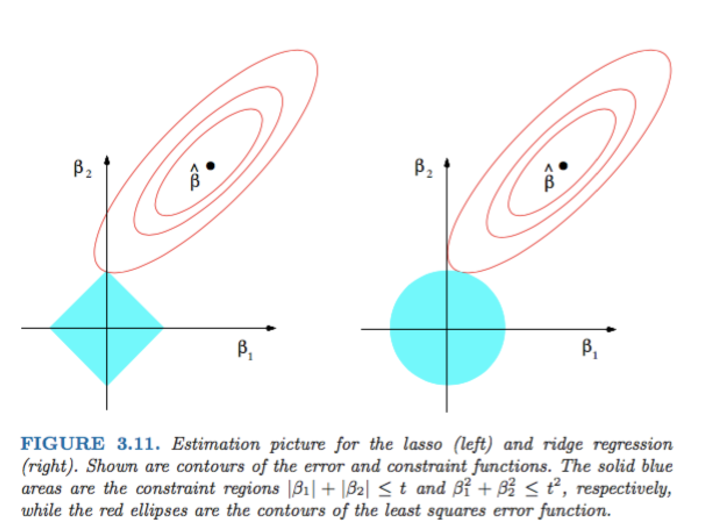
\includegraphics[width=\linewidth]{../img/regularization.png}
  \caption{$L^1$ and $L^2$ regularizaiton.}
  \label{reg}
  \end{figure}
 
Let $\beta = (\beta_1, \beta_2)$ be the desired coefficients in a linear regression so that we seek to minimize
\begin{equation}
\mathcal{L}(\beta) := \frac{1}{N} \sum_{i=1}^N (y_i - \beta_1 x_{i1} - \beta_2 x_{i2})^2.
\end{equation}

Recall that we wish to penalize the size of the coefficients in order to not over fit our model, so we impose a constraint on the size of $\beta$. More precisely, we seek to solve the \textbf{constrained optimization problem:}
\begin{align}
\min_{\beta}\; &\mathcal{L}_{\lambda} (\beta) \\
|\beta_1|^p + |\beta_2|^p &\leq C,
\end{align}

for $p=1, 2$. \\\\

\textbf{Common Question:} Why do we choose $p=1$ or $p=2$? Why not some other p?\\\\

\textbf{Answer:} 
\begin{itemize}
\item The norm $L^2$ (ie. $p=2$ )  is very well behaved and is related to the equation for a sphere ($x^2+y^2 = r^2$). Recall that we have an exact solution to the linear regression problem, ie. (1.1), when we choose our norm
to be $L^2$ (as we have above, known as ordinary least squares - there is no exact solution if we replace the exponent $2$ in (1.1) with a $1$). 
\item The constant surfaces of $L^2$ (level surfaces, ie. where $x^2 + y^2 = r^2$) are the surfaces of constant distance from the origin.
\item Thinking of a convex function $f(x) = x^2$, this has a constant second derivative $f''(x) = 2$ so it's \textbf{uniformly convex} - meaning we have stability, uniqueness, etc when minimizing with respect to this norm generally.
\item $p=1$ is rather unique in that it provides a way of \emph{regularizing which results in sparse coefficients } (ie. many zero coefficients, allowing you to choose the most important features). This is explained in these notes below.
\item There isn't really any other advantage to using some other $L^p$ space for $p > 2$, yet many disadvantages (such as degeneracy). 
\end{itemize}

Let's define $g(\beta) = |\beta_1|^p + |\beta_2|^p$, and for now, focus on $p=2$. Referring to the figure on the right below, we seek to minimize (1.1) with some constraint
\[ \beta_1^2 + \beta_2^2 \leq C.\]

The size of the constraint depends on how strong we want our regularization to be, and we choose the constant $C$ which gives the best performance on test data (as in lecture). More on this below.\\\\


How do we minimize this? Imagine to fix ideas that $C=1$ so that $\beta_1^2 + \beta_2^2 \leq 1$, and we seek to solve
\begin{align}
\min_{\beta} \; &\mathcal{L}_{\lambda} (\beta) \\
\beta_1^2 + \beta_2^2 &\leq 1.
\end{align}

\section{Derivation of Lagrange Multipliers}

The following facts will make the above clear:
\begin{itemize}
\item $ \beta \mapsto \mathcal{L}(\beta)$ is constant along \emph{level sets} (ie. where $\mathcal{L}(\beta) = \textrm{ constant } $) by definition.
\item $ \beta \mapsto \mathcal{L}(\beta)$ changes only in the direction \textbf{orthogonal} to the level sets, and this is given by $\nabla_{\beta} \mathcal{L}(\beta)$. This is clear because
in any direction along the surface, $\mathcal{L}$ is constant. 

\item \textbf{Case 1:} If $\nabla \mathcal{L}(\beta_0) = 0$ for some $\mathbf{\beta^0}$ in $\beta_1^2 + \beta_2^2 < 1$ then we solve as we do in normal calculus. 
\item  \textbf{Case 2:} If $\nabla \mathcal{L}(\beta_0) \neq 0$ in $\beta_1^2 + \beta_2^2 < 1$. Then the minimum occurs on the boundary of $\beta_1^2 + \beta_2^2$. This is the Lagrange multiplier case.
\item Recall the vector orthogonal to the level set is the gradient vector. So if $g(\beta_1,\beta_2) = \beta_1^2 + \beta_2^2$, then the orthogonal vector to the surface $\beta_1^2 + \beta_2^2$ is in the direction
of $\nabla g = 2\langle \beta_1, \beta_2 \rangle$.
\item \textbf{Main Point:} The minimum of $\mathcal{L}$ has to occur at a point where $\nabla \mathcal {L}$ is in the same direction as $\nabla g$. If it weren't, then we could move along the surface $\beta_1^2 + \beta_2^2$ a bit
to decrease the value (try drawing a picture or looking at the figures), so it wouldn't be a minimum!.
\end{itemize}

From the above points, we conclude that the minimum occurs at some point $\langle \beta_1^*, \beta_2^* \rangle$ such that
\[ \nabla \mathcal{L}(\beta_1^*, \beta_2^*) = \lambda \nabla g(\beta_1^*, \beta_2^*). \]

\section{Interpreting Lasso and Ridge regression}

Observing the figure on the right, when we have $\beta_1^2 + \beta_2^2 \leq C$, we see the minimum has an equal chance of hitting the level set of $\beta_1^2 + \beta_2^2 = C$ at any point. As a result,
the errors are generally equally distributed amongst the coefficients $\beta_1$ and $\beta_2$.\\\\

On the other hand, when $|\beta_1| + |\beta_2| = C$, we see that the level set of $\mathcal{L}$ is most likely to be tangent to the level sets (diamonds) at a corner  (ie. where $\beta_1=0$ or $\beta_2=0$),
\textbf{since there are only 4 possible directions where both of the coefficients are non-zero, making it highly unlikely that the level sets of $\mathcal{L}$ has a tangent parallel to any one of these directions. }\\\\


\textbf{Conclusion:} As a result, Lasso tends to result in \emph{sparser} coefficients (ie. many zero coefficients), while Ridge generally distributes the error more evenly among the coefficients. 

\section{How much of a constraint do we use?}

Recall from lecture that we want to train a model by solving the problem:

\begin{align}
\min_{\beta}\; &\mathcal{L}_{\lambda} (\beta | (x_i,y_i) = \textrm{ training data }) \\
&|\beta_1|^p + |\beta_2|^p \leq C.
\end{align}

Let's denote $\beta_C$ as the solution to the above constrained optimization problem (note it depends on $C$), so that our model is
\[ f_C(x) = \beta_{C} \cdot x.\]

 Then the optimal C, denoted $C^*$ is determined by

\begin{equation}
C^* = \textrm{argmin}_C \frac{\sum_{i=1}^N (y_i - f_C(x_i))^2}{\sum_{i=1}^N (y_i - \bar y)^2}.
\end{equation}
\end{document}